\Needspace{0.72\textheight}
\section{Conjectural log-concavity}\label{sec:log-concavity-conjecture}

We state the following conjecture on Euler characteristics near slope one.
See \cite{CDW, Oko} for related studies and
\cite[Section 1.12]{Oka2026} for a study of log-concavity
in mathematics and statistical mechanics.

\begin{conjecture}[Euler-characteristic ratios near slope one]\label{conj:central-ratio-log-concavity}
Let $a\in\Z_{\ge5}$ satisfy $\gcd(a,6)=1$. Then,
\[
 \frac{E_3(a,a+4)}{E_3(a,a+3)}
 \le
 \frac{E_3(a,a+3)}{E_3(a,a+2)}.
\]
\end{conjecture}

We provide the following figure on Conjecture~\ref{conj:central-ratio-log-concavity}.

\begin{figure}[H]
\centering
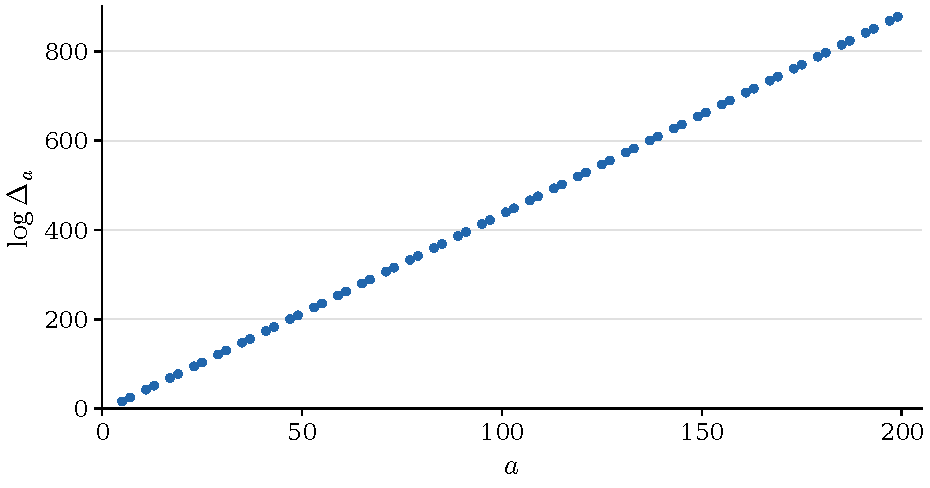
\includegraphics[width=0.9\textwidth]{figures/conjecture-delta-log.pdf}
\caption[Logarithms of the log-concavity differences]{Let
$\Delta_a=E_3(a,a+3)^2-E_3(a,a+2)E_3(a,a+4)$.
The points plot $\log\Delta_a$ by explicit computation for
$a\in[5,200]_{\Z}$ satisfying $\gcd(a,6)=1$.
All 66 differences are positive.}
\label{fig:conjecture-delta-log}
\end{figure}
